%%% Local Variables:
%%% TeX-master: "eunchurn_park"
%%% End:
\cvevent{\printinfo{\faPlusSquare}{AD.Fi 플랫폼 개발}}{(주)단비코리아 개발리딩}{2020.01 -- 2022.06}{Seoul, Korea}

\label{adfi}

\begin{itemize}[label=\emoji{satellite}]
	\item 소개: 인터넷 WiFi 공유기 광고 시스템(매장 광고 송출, 광고 관리, 매장, 브랜드, 영업사원, 대리점, 총판 관리) 개발
	\item 개발 기간: 6개월
	\item 유지관리 기간: 18개월
	\item 개발 인원: 5명
	\item 개발한 서비스
	      \begin{itemize}[label=\emoji{pushpin}]
		      \item 공유기 광고 송출 페이지: Captive Portal 광고 노출 및 인터넷 연결 허용
		            \begin{figure}[!ht]
			            \begin{fullwidth}
				            \parbox{0.8\textwidth}{
					            \centering
					            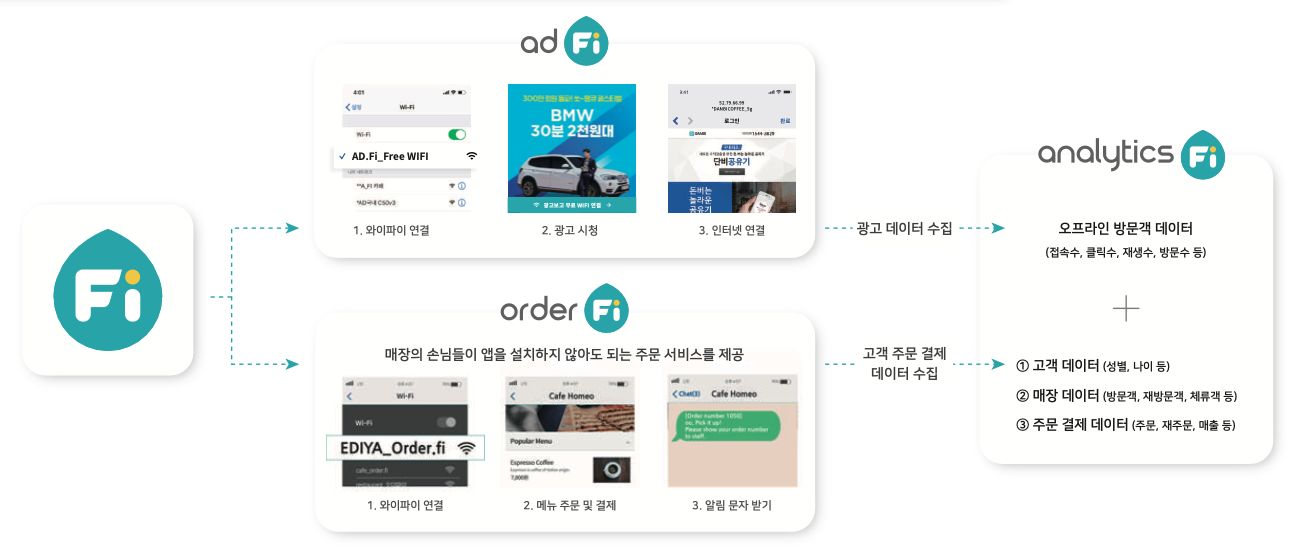
\includegraphics[width=0.8\textwidth]{images/ad-fi-platform.png}
					            \caption*{Fi 솔루션 개발}
				            }\qquad
				            \parbox{0.68\textwidth}{
					            \centering
					            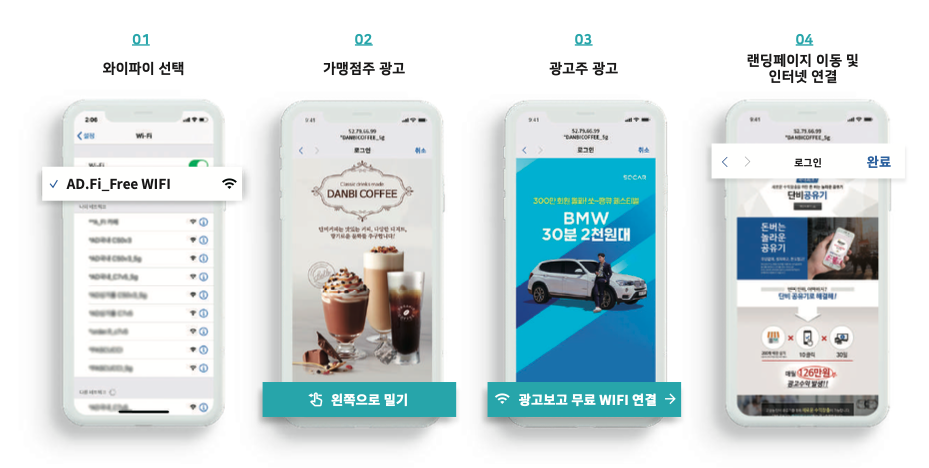
\includegraphics[width=0.68\textwidth]{images/ad-fi.png}
					            \caption*{공유기 광고 송출}
				            }
			            \end{fullwidth}
		            \end{figure}
		      \item 광고 집계 및 광고 관리 백오피스: 매장주, 영업사원, 대리점, 총판, 브랜드, 브랜드그룹 어드민
		            \begin{figure}[!ht]
			            \begin{fullwidth}
				            \parbox{0.35\textwidth}{
					            \centering
					            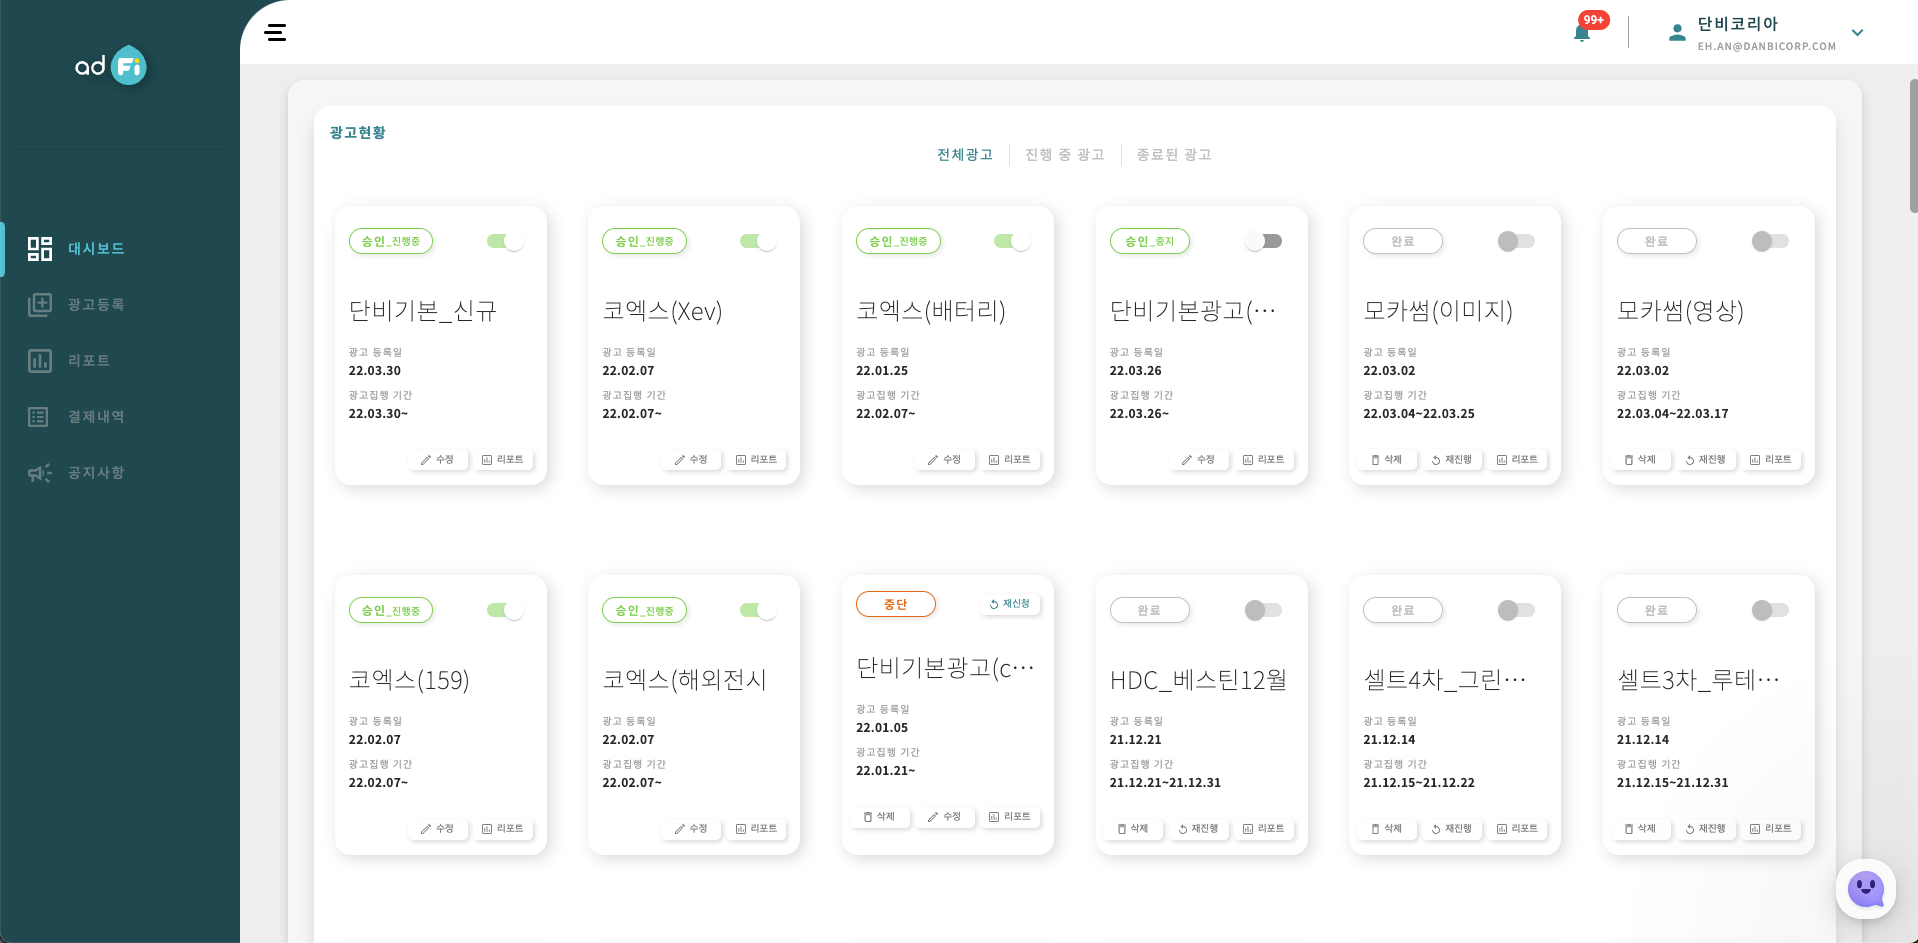
\includegraphics[width=0.35\textwidth]{images/ad-fi-admin-ad-dashboard.png}
					            \caption*{광고 송출 현황}
				            }\qquad
				            \parbox{0.35\textwidth}{
					            \centering
					            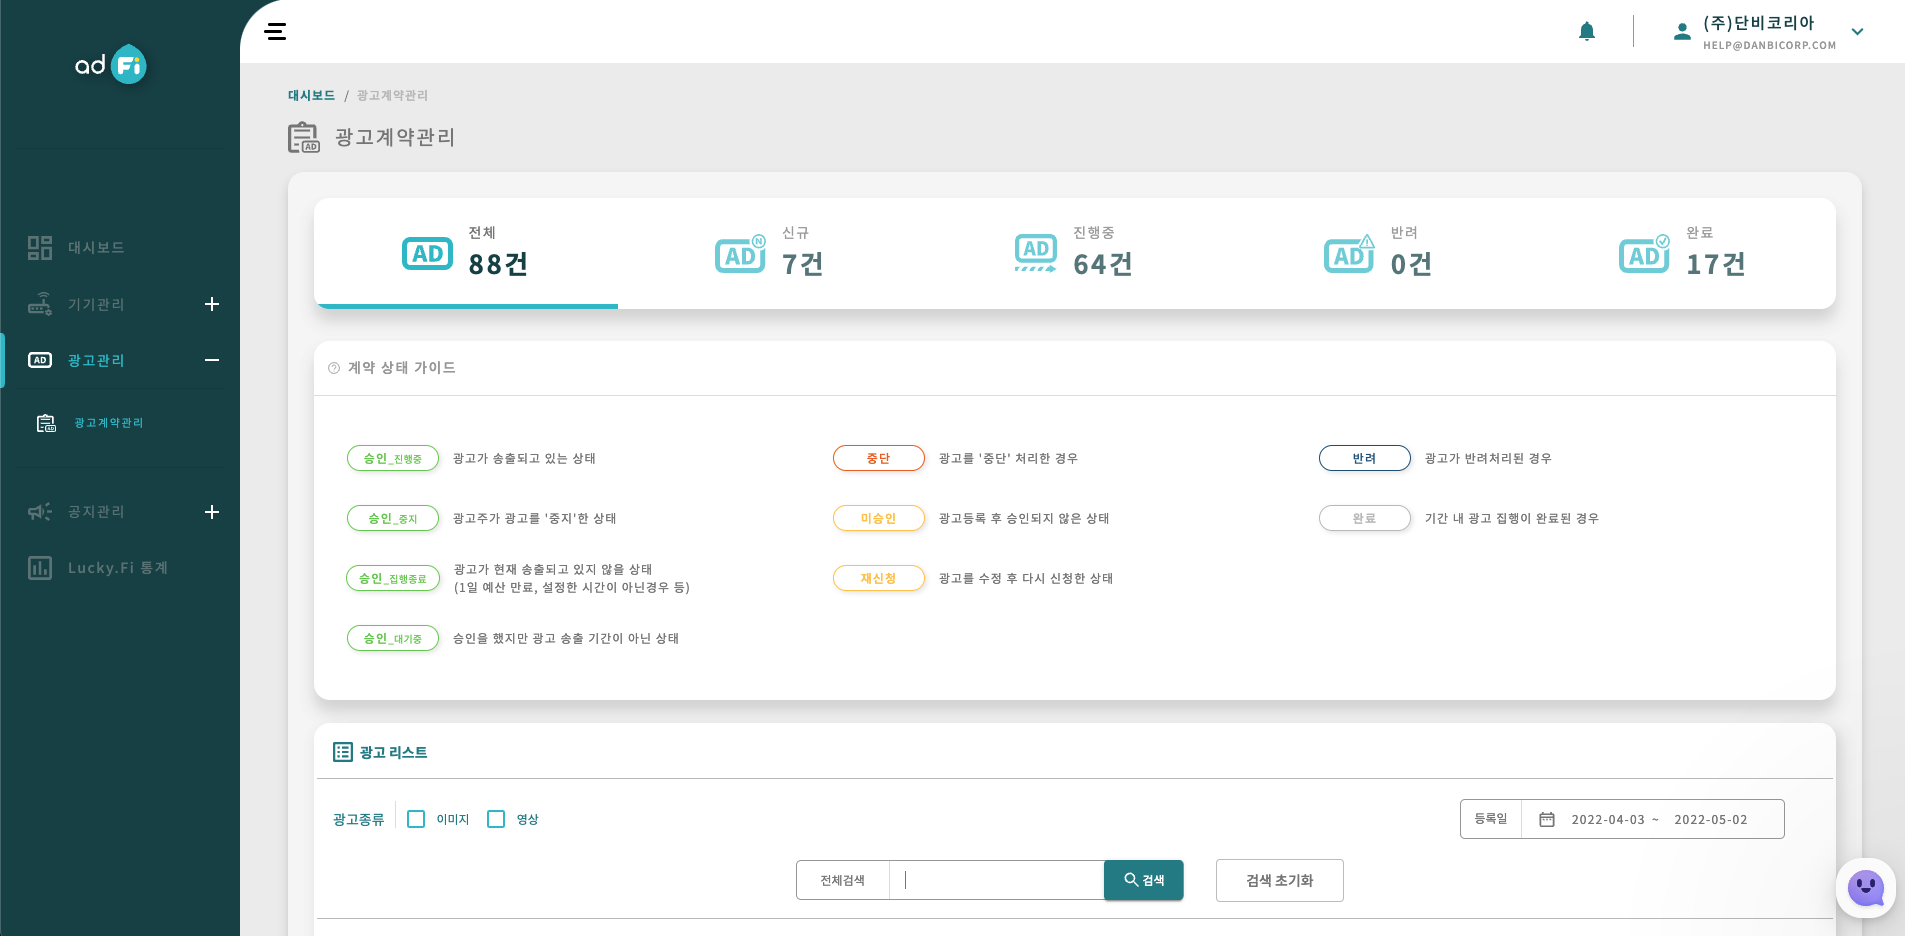
\includegraphics[width=0.35\textwidth]{images/ad-fi-admin-ad-manage.png}
					            \caption*{광고 관리}
				            }\qquad
				            \parbox{0.35\textwidth}{
					            \centering
					            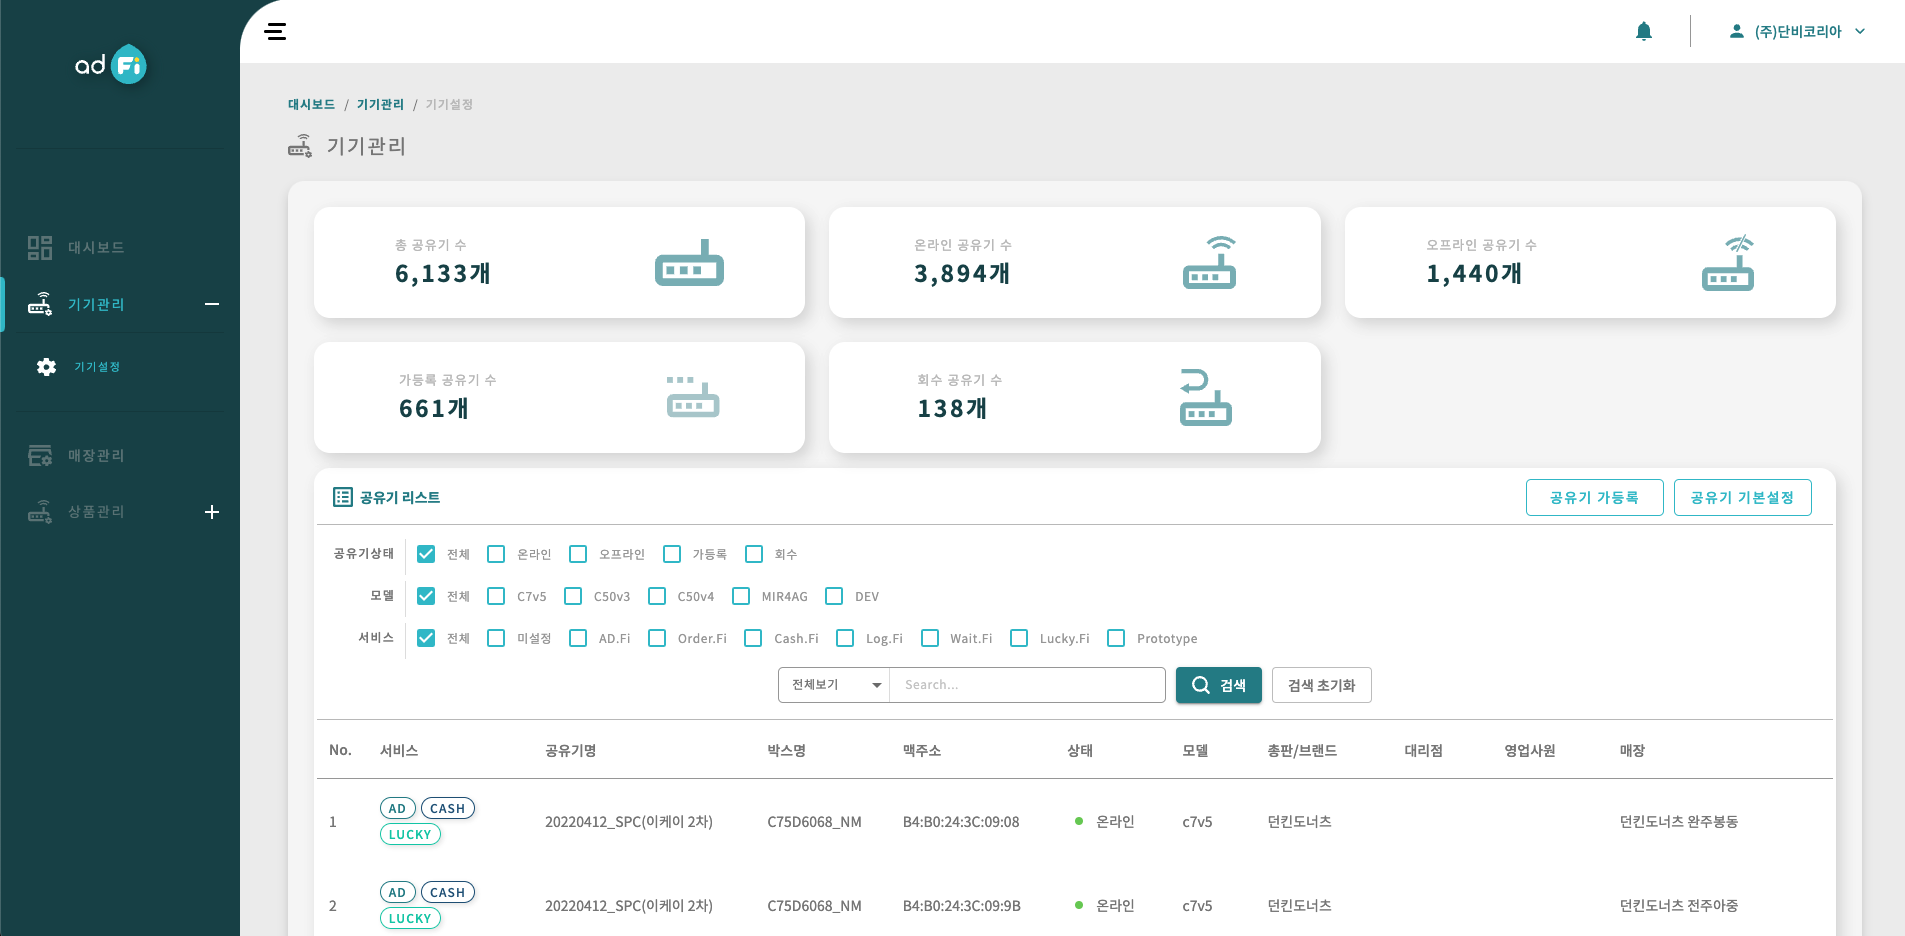
\includegraphics[width=0.35\textwidth]{images/ad-fi-admin-device-manage.png}
					            \caption*{공유기 기기 관리}
				            }\qquad
				            \parbox{0.35\textwidth}{
					            \centering
					            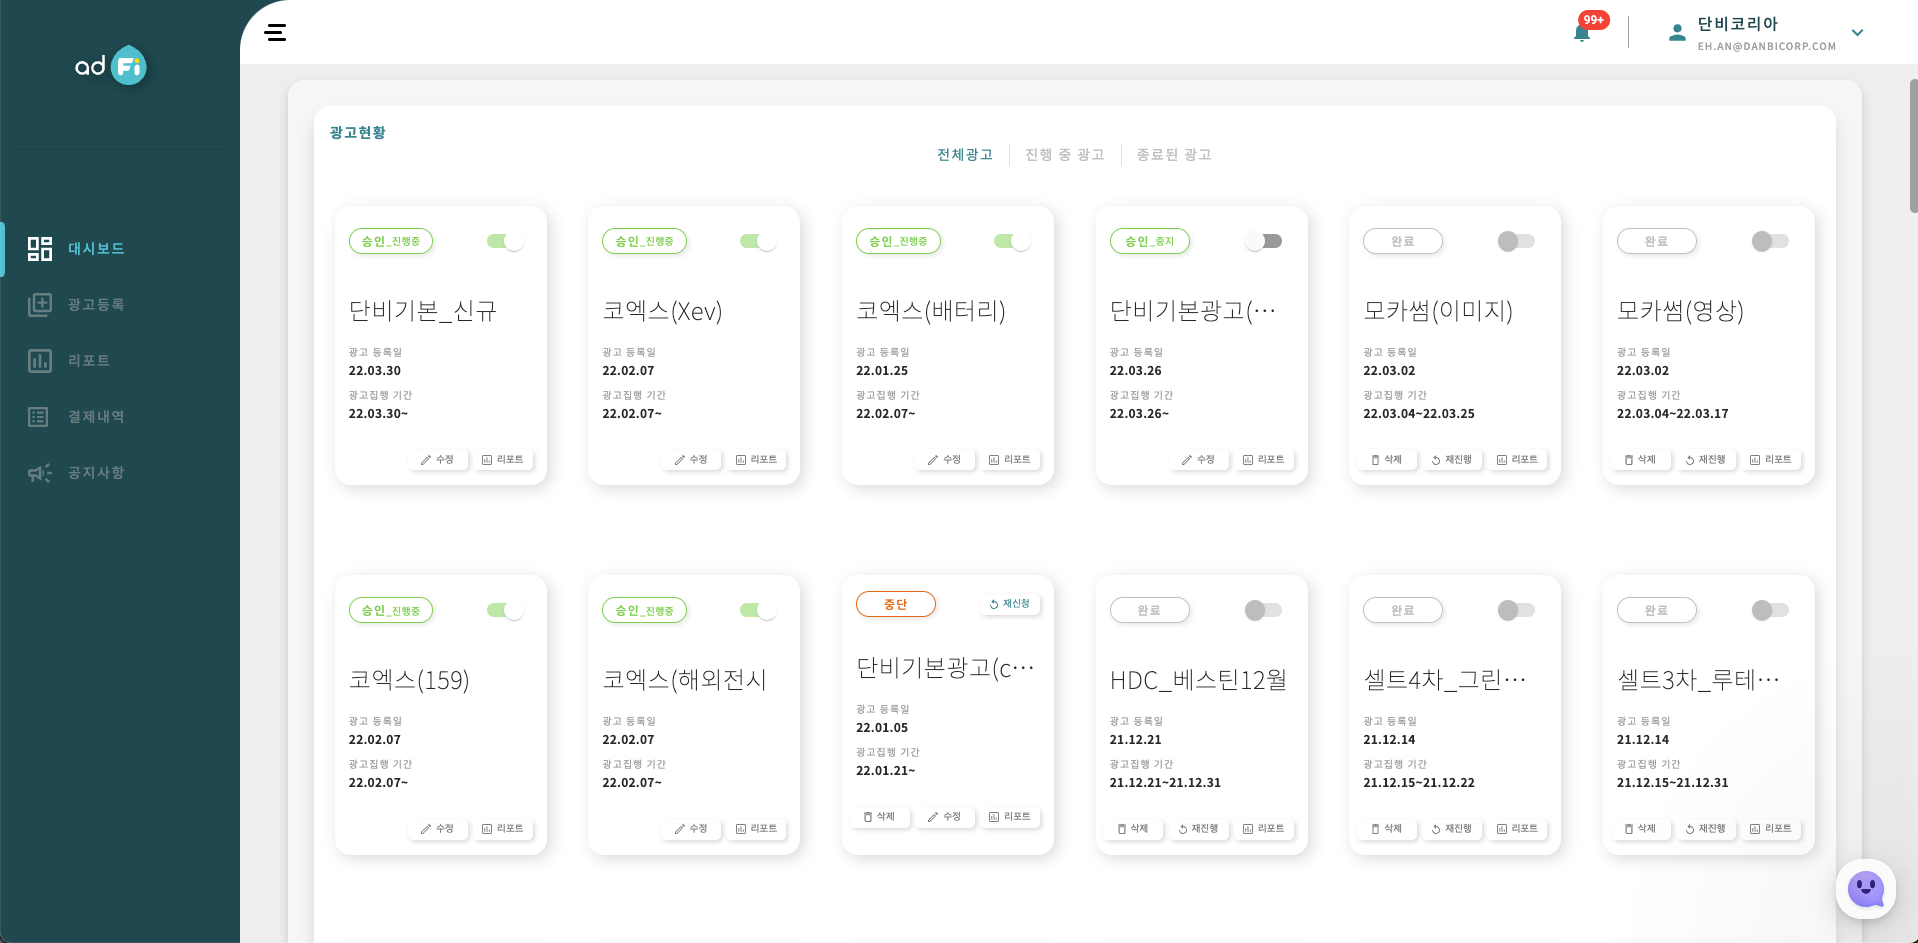
\includegraphics[width=0.35\textwidth]{images/ad-fi-admin-ad-dashboard.png}
					            \caption*{광고 송출 현황}
				            }
				            \parbox{0.35\textwidth}{
					            \centering
					            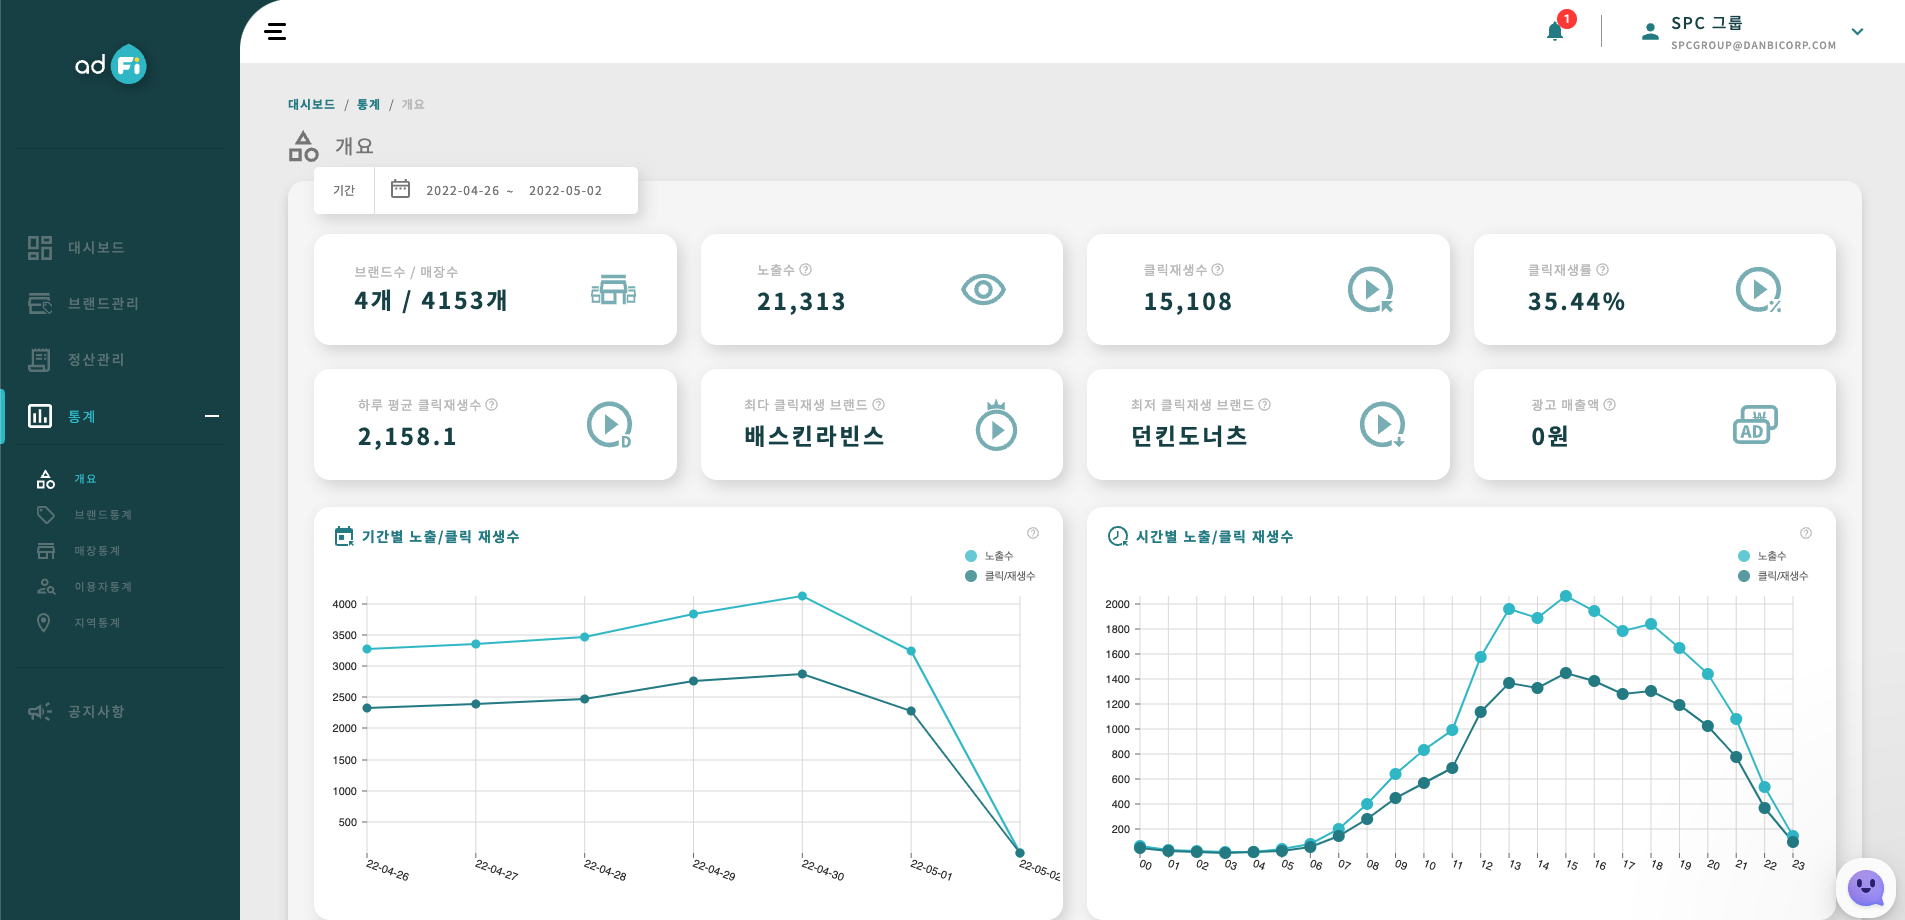
\includegraphics[width=0.35\textwidth]{images/ad-fi-admin-dashboard.png}
					            \caption*{대시보드: 통계}
				            }\qquad
				            \parbox{0.35\textwidth}{
					            \centering
					            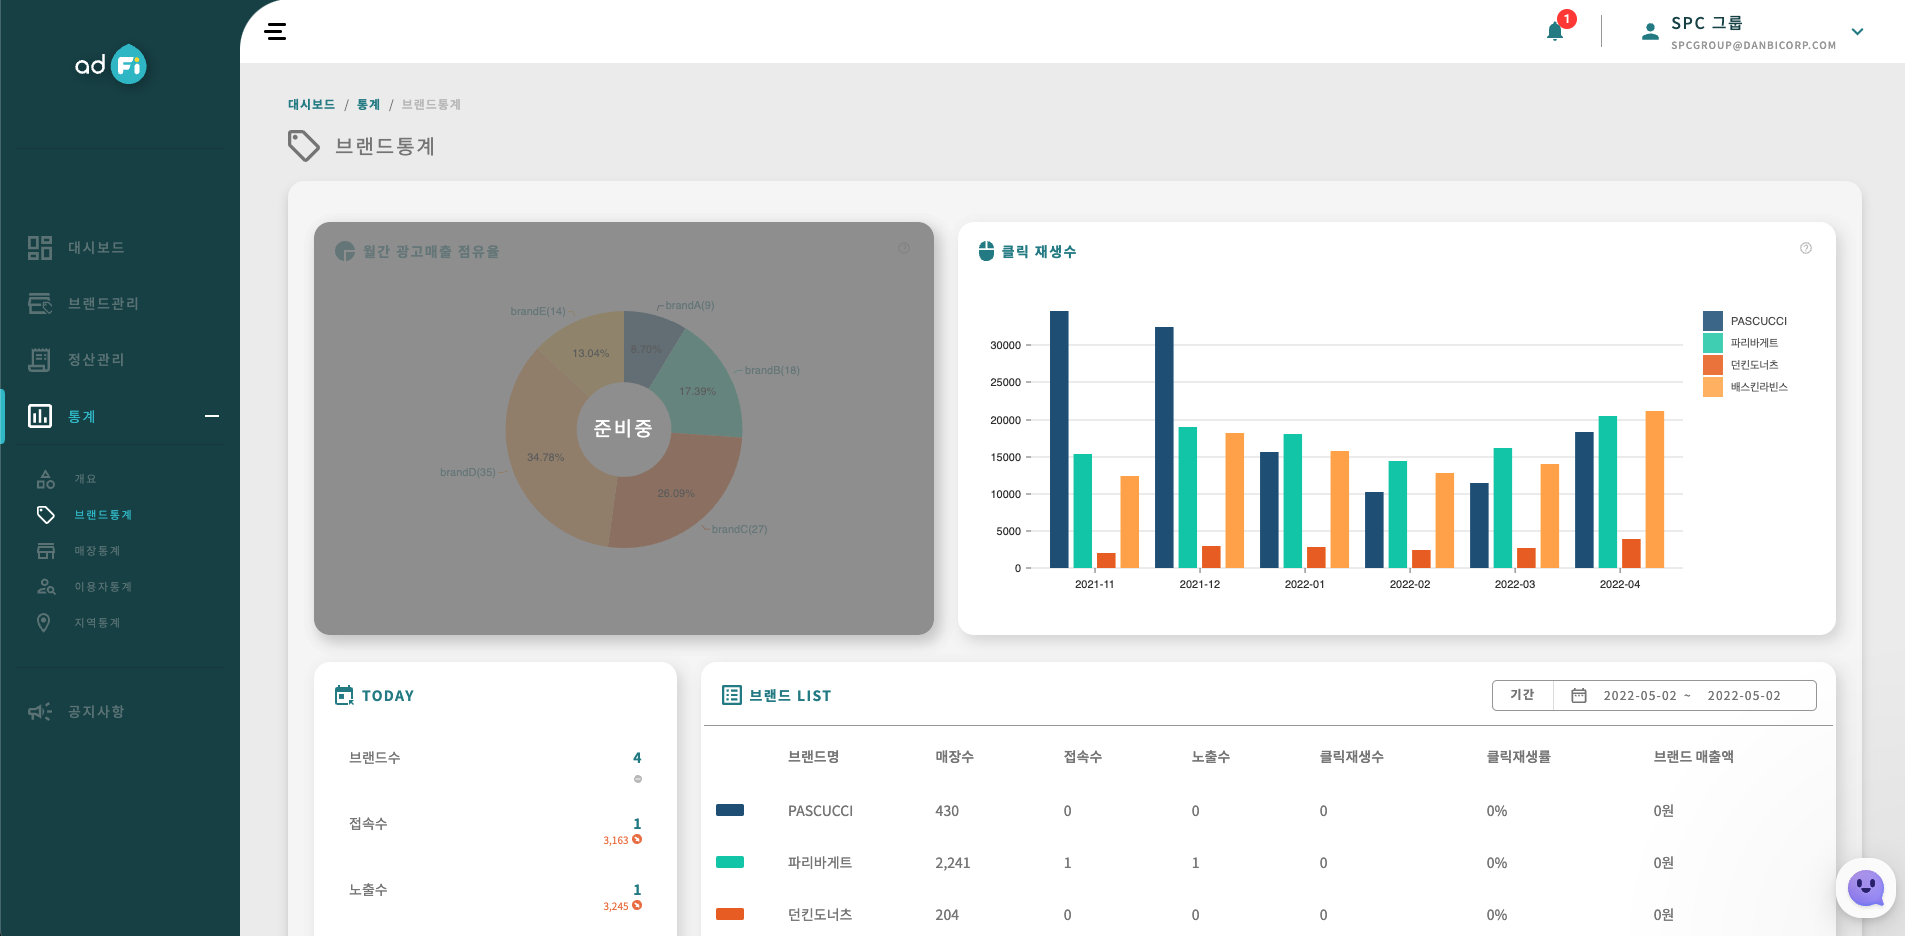
\includegraphics[width=0.35\textwidth]{images/ad-fi-admin-brand-stat.png}
					            \caption*{브랜드 어드민: 통계}
				            }\qquad
				            \parbox{0.35\textwidth}{
					            \centering
					            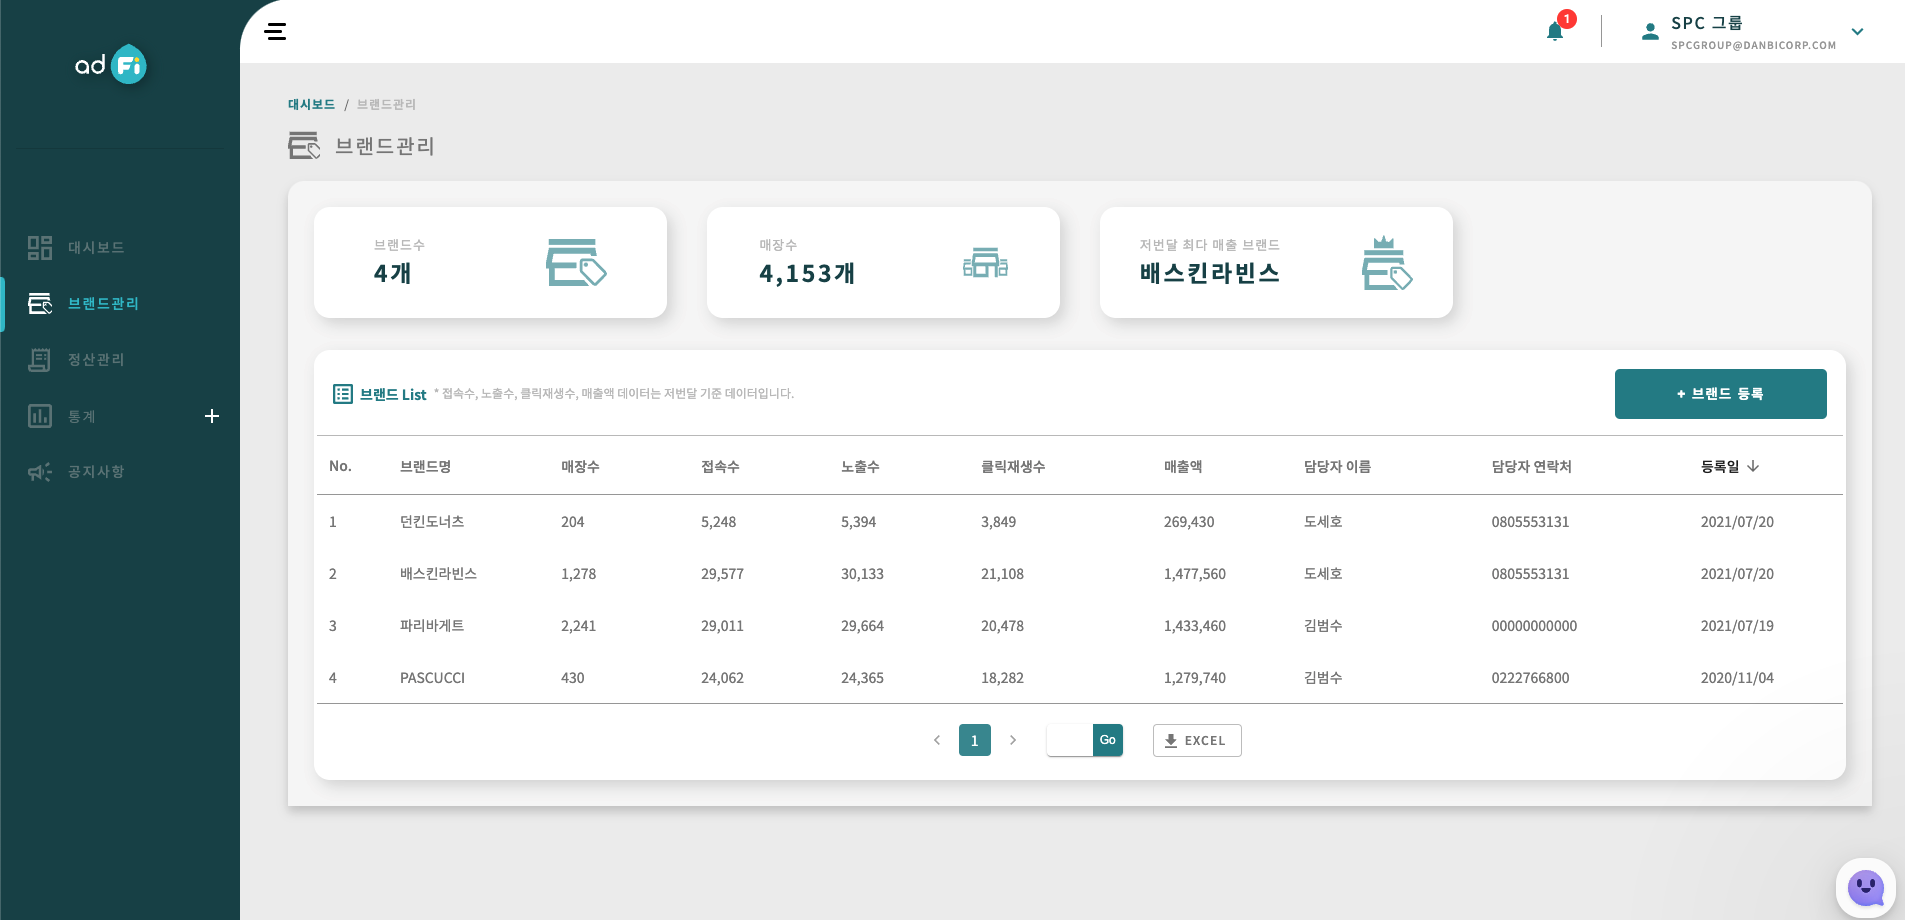
\includegraphics[width=0.35\textwidth]{images/ad-fi-admin-brand.png}
					            \caption*{브랜드 관리}
				            }\qquad
				            \parbox{0.35\textwidth}{
					            \centering
					            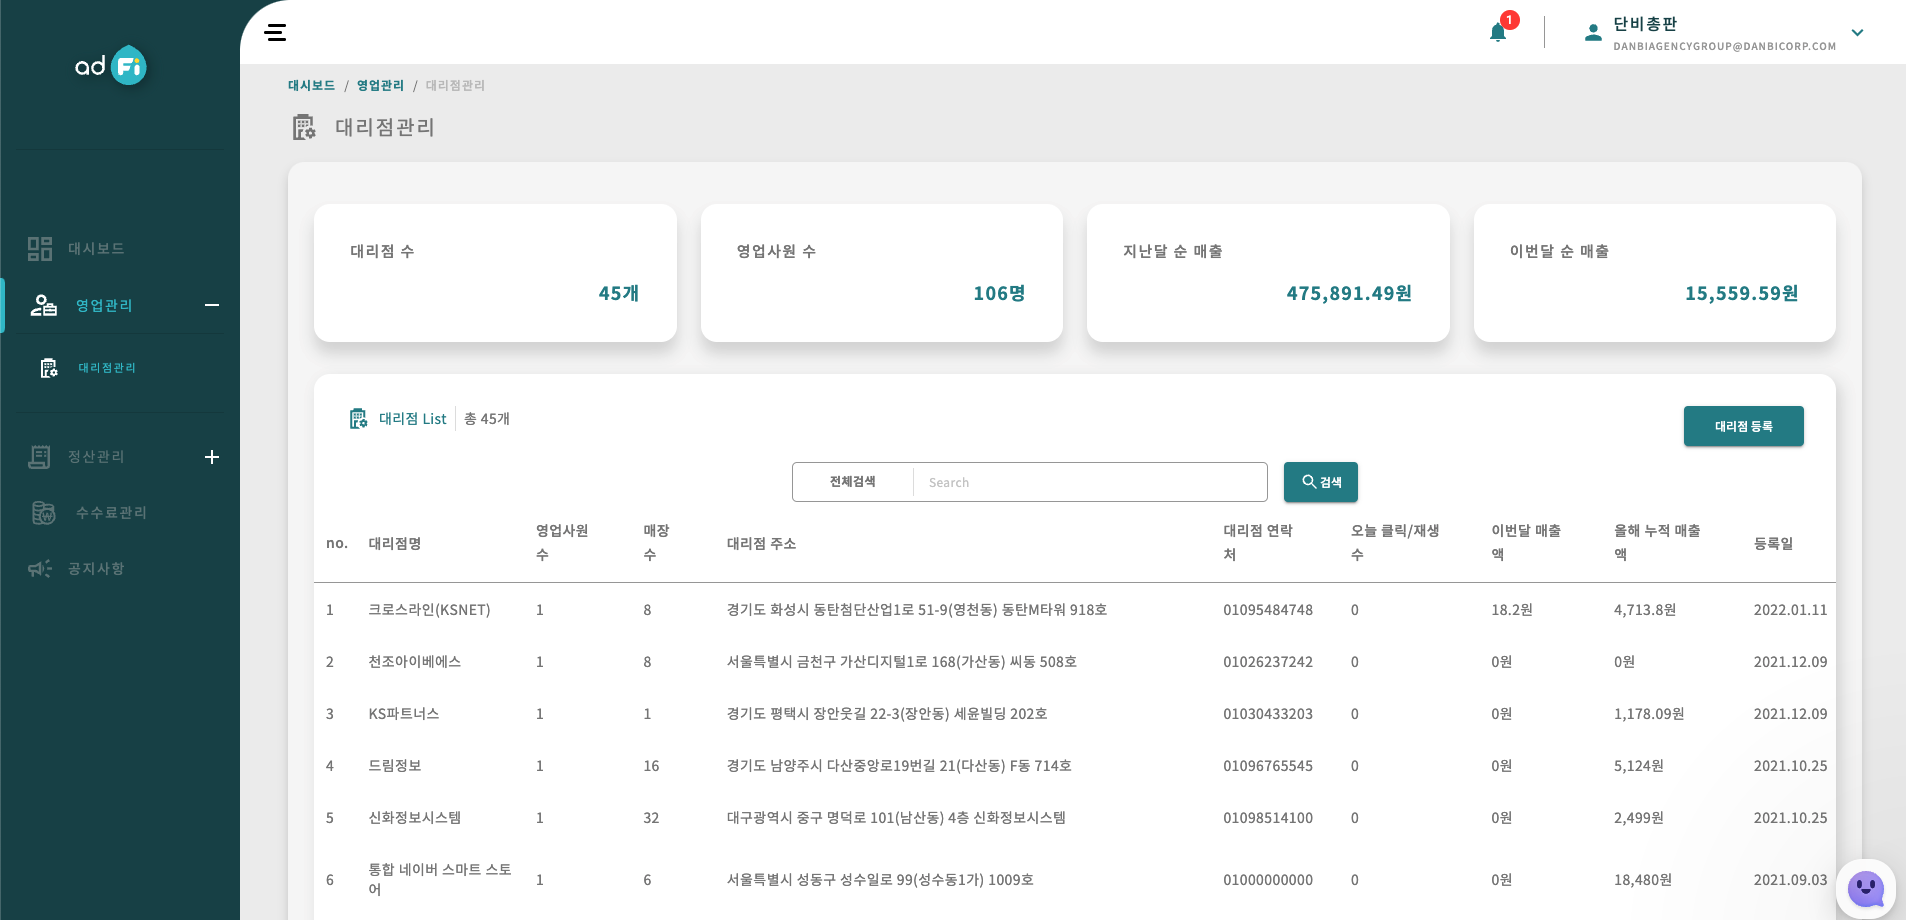
\includegraphics[width=0.35\textwidth]{images/ad-fi-admin-agency.png}
					            \caption*{대리점 관리}
				            }
			            \end{fullwidth}
		            \end{figure}
		      \item 타겟광고 트래킹 시스템 개발
		      \item 인프라 구성:
		            \begin{figure}[!ht]
			            \begin{fullwidth}
				            \parbox{1.6\textwidth}{
					            \centering
					            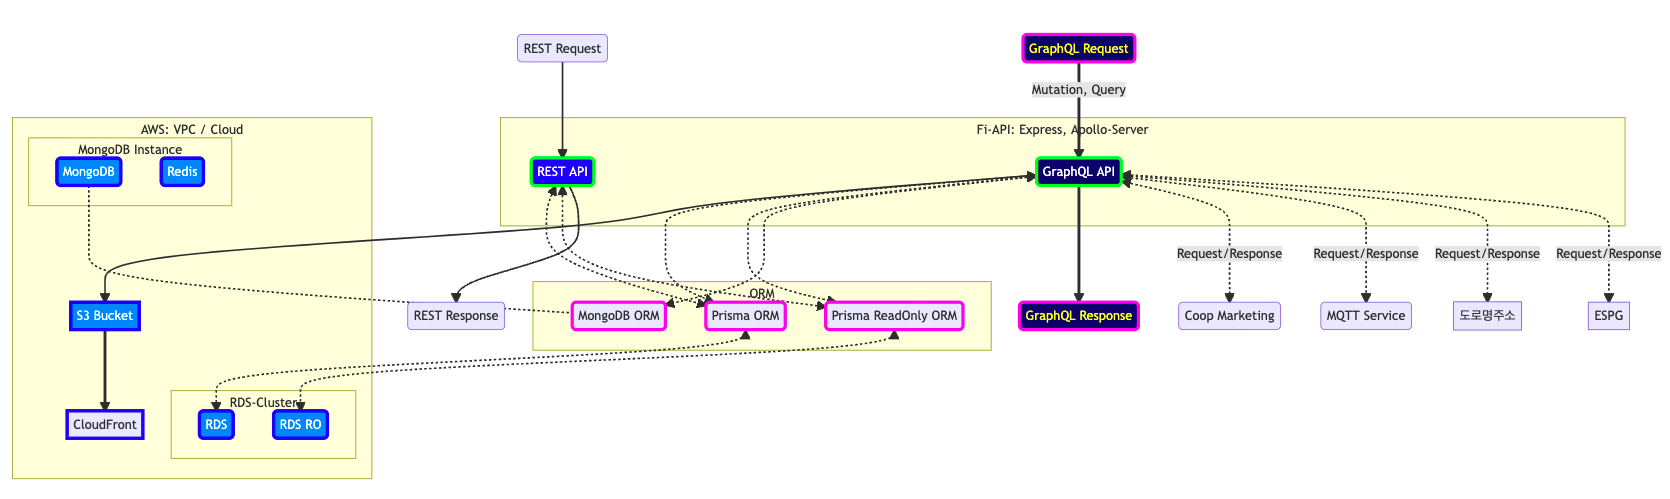
\includegraphics[width=1\textwidth]{images/architecture-fi.png}
					            \caption*{AWS 인프라 구성}
				            }
			            \end{fullwidth}
		            \end{figure}
		            \begin{itemize}
			            \item AWS EC2, CodePipeline, AutoScalingGroup, S3, Lambda
			            \item Linux system daemon(systemd) and timer
			            \item Docker swarm stack: Microservice containers
		            \end{itemize}
		            \begin{figure}[!ht]
			            \begin{fullwidth}
				            \parbox{1.6\textwidth}{
					            \centering
					            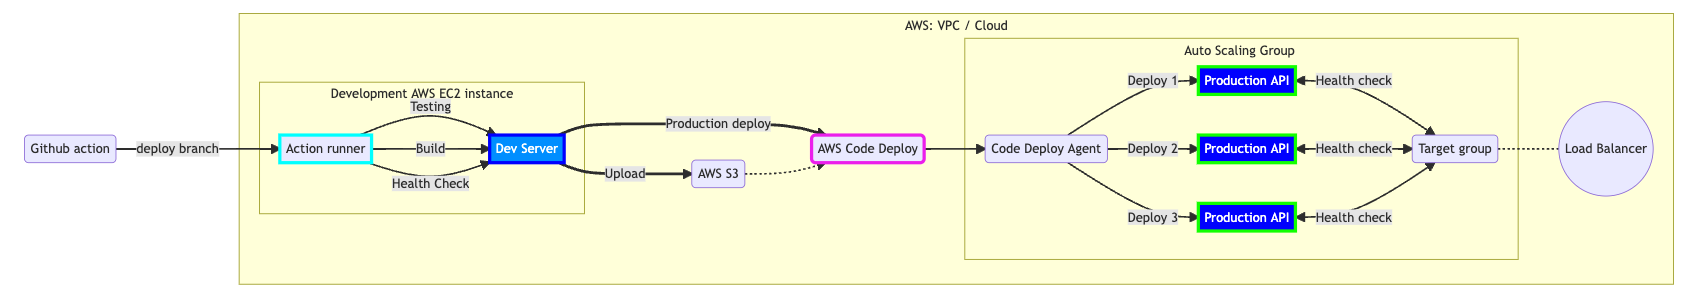
\includegraphics[width=1.6\textwidth]{images/deployment-pipeline.png}
					            \caption*{AWS 배포 파이프라인}
				            }
			            \end{fullwidth}
		            \end{figure}
		      \item 백엔드 개발 스택
		            \begin{itemize}
			            \item Type-safe pipeline: TypeScript, NodeJS, Express, Apollo Server, Prisma ORM, Nexus GraphQL, Open API Spec. v3
			            \item Code-first GraphQL schema: Nexus-GraphQL
			            \item Asynchronosus API: Mosquitto, MQTTjs, Async API
		            \end{itemize}
		      \item 프론트 개발 스택
		            \begin{itemize}
			            \item TypeScript, ReactJS, Context API, Material UI, Styled Component, JSS
			            \item GraphQL-codegen(React, Apollo-client)
		            \end{itemize}
		            \begin{figure}[!ht]
			            \begin{fullwidth}
				            \parbox{1.6\textwidth}{
					            \centering
					            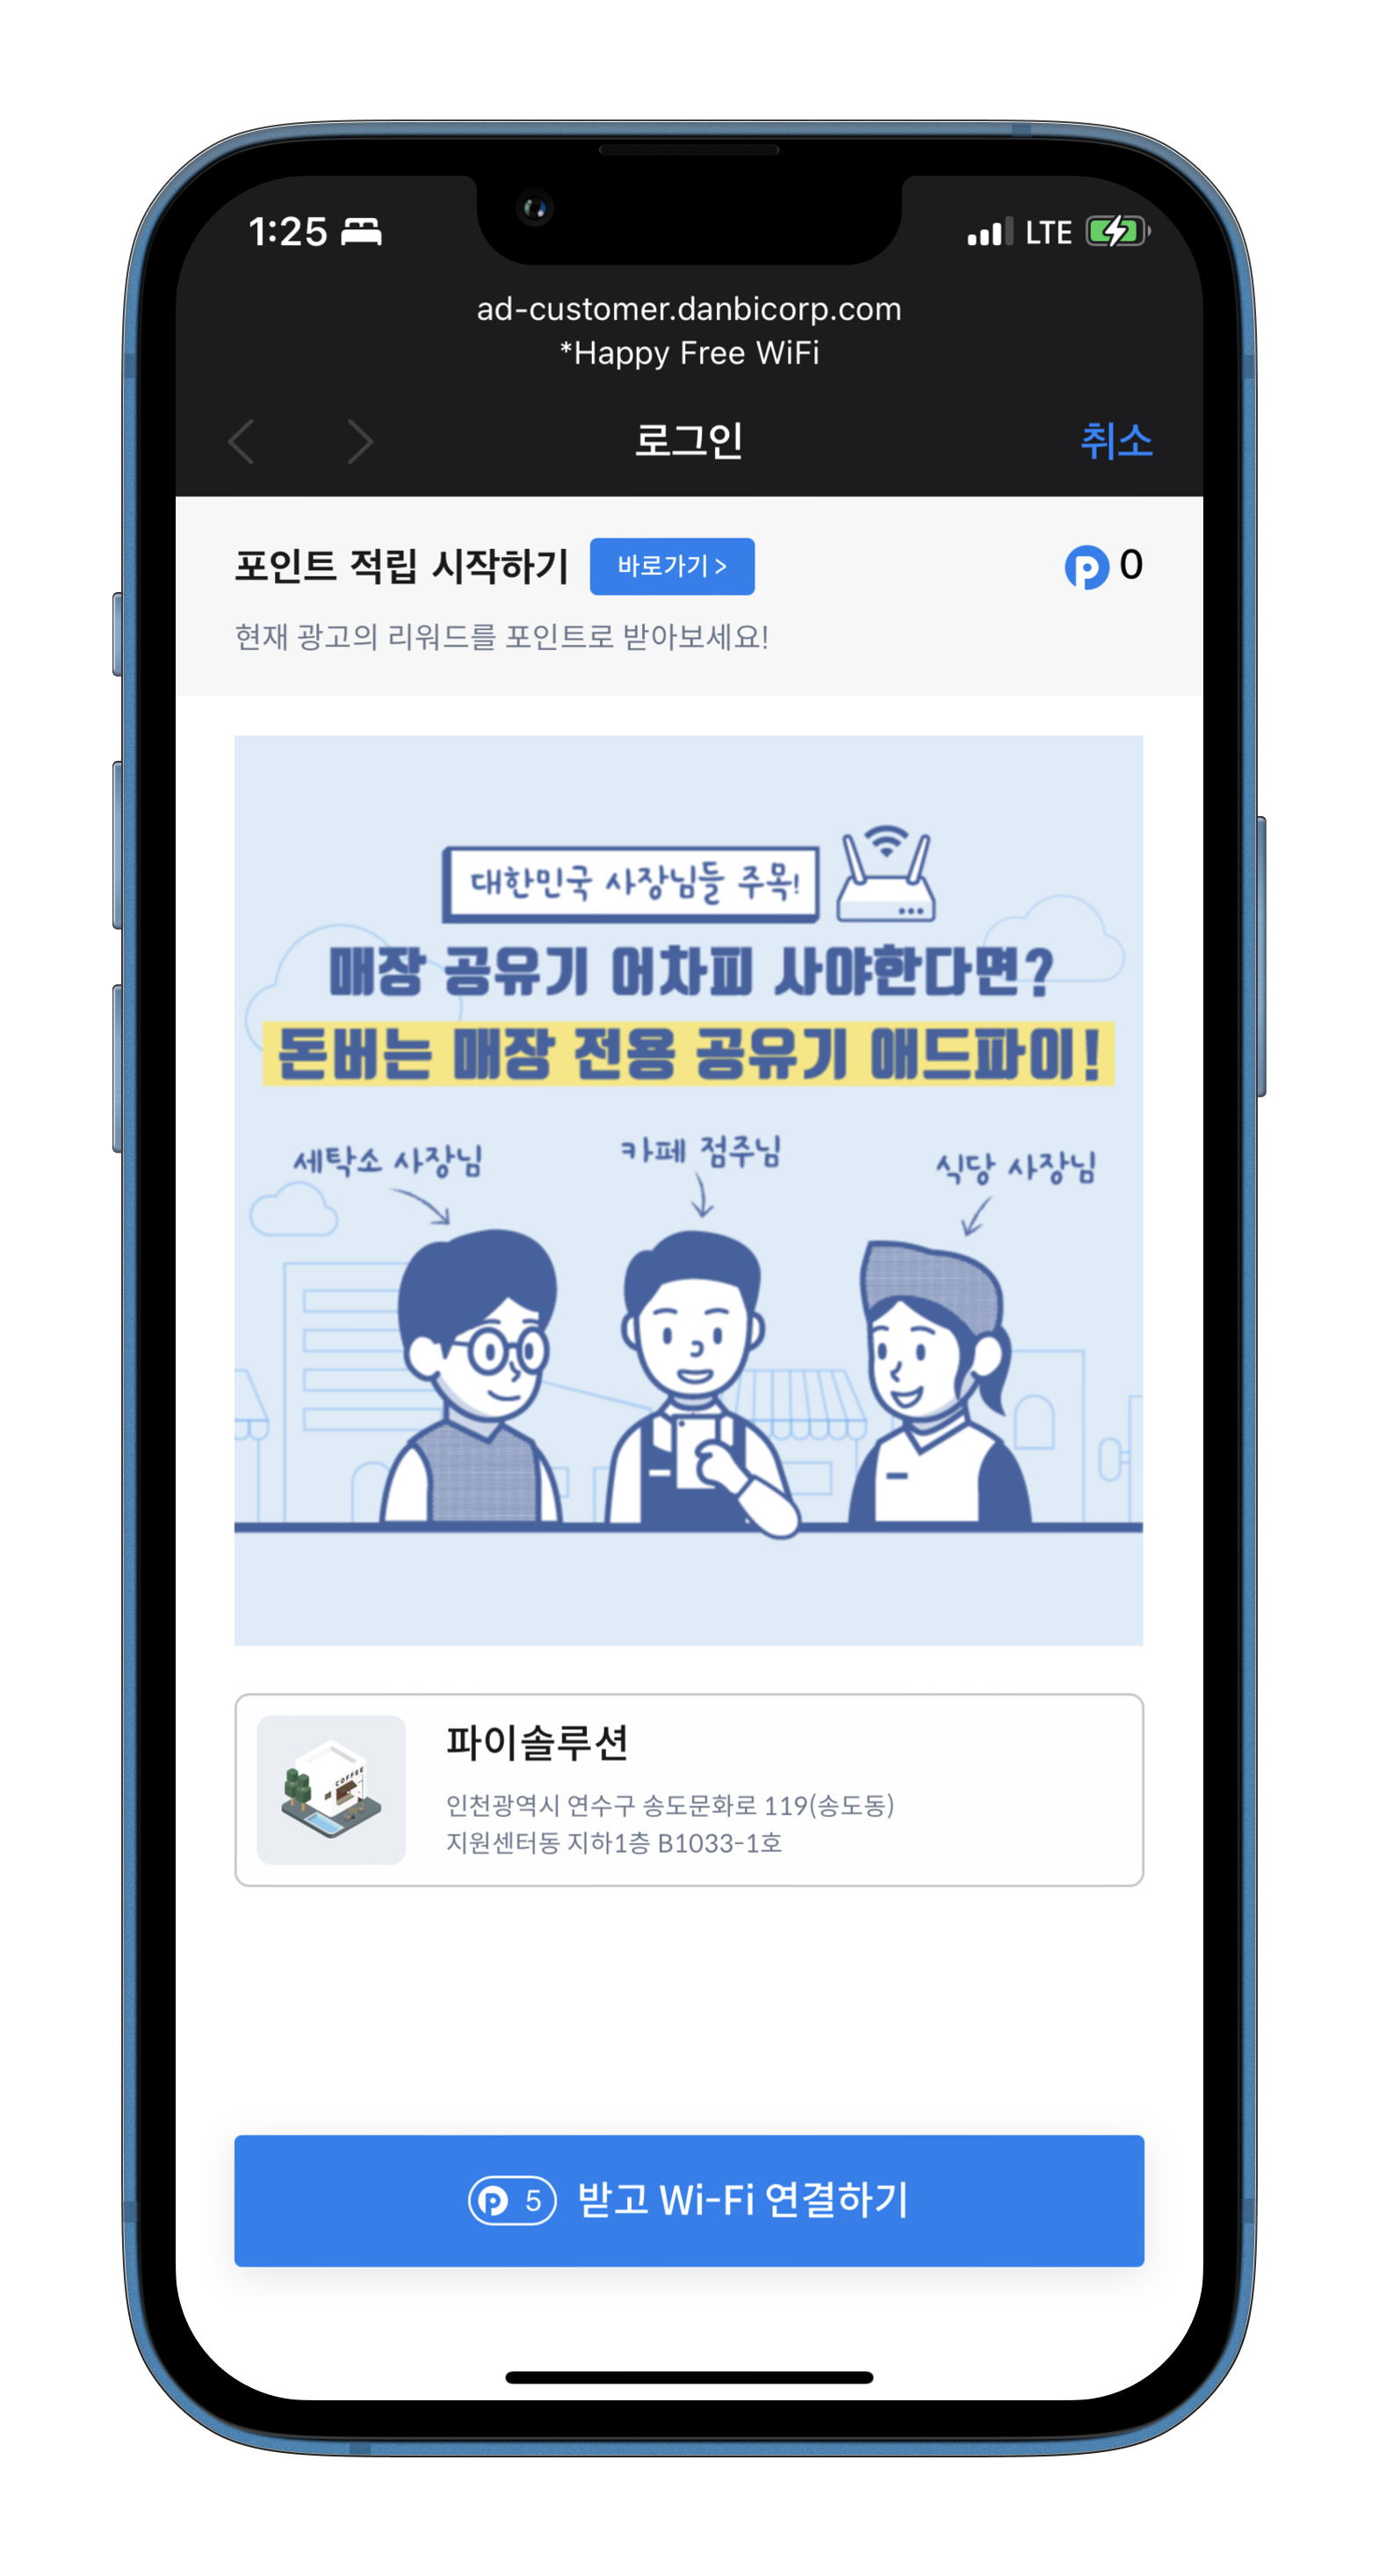
\includegraphics[width=0.3\textwidth]{images/ad-fi-reward.png}
					            \caption*{AD.Fi Captive portal}
				            }
			            \end{fullwidth}
		            \end{figure}
	      \end{itemize}

\end{itemize}

\cvevent{\printinfo{\faPlusSquare}{Log.Fi(매장 코로나 19 방명록) 개발}}{(주)단비코리아}{2020.06 -- 2020.06}{Seoul, Korea}

\label{logfi}

\begin{itemize}[label=\emoji{satellite}]
	\item 소개: 코로나19로 인한 팬데믹 상황 초기에 매장 방명록을 손으로 작성하는 사태를 막기 위해 공유기 Captive portal 브라우저를 활용하여 방문자 기록을 할 수 있도록 함
	\item 개발 기간: 5일
	\item 개발 인력: 1인
	\item 개발한 서비스
	      \begin{itemize}[label=\emoji{pushpin}]
		      \item 체크인 페이지: Captive Portal 브라우저에서 방문자 기록
		      \item 어드민 개발: 사용자 리스트
		      \item 이후 공유기 설정 및 등록 페이지로 활용, 공유기 가등록 및 판매
	      \end{itemize}
\end{itemize}

\cvevent{\printinfo{\faPlusSquare}{Lucky.Fi(매장 경품추첨 앱) 개발}}{(주)단비코리아 개발리딩}{2021.06 -- 2021.07}{Seoul, Korea}

\label{luckyfi}

\begin{itemize}[label=\emoji{satellite}]
	\item 소개: AD.Fi 서비스에서 광고를 시청하고 인터넷을 사용하기전 사용자에게 리워드를 지급하기 위한 서비스. 당첨자를 특정할 수 있는 서비스이며 이를 통해 AD.Fi의 타겟 광고를 유용하게 하기 위함
	\item 개발 기간: 4주
	\item 개발 인력: 5인
	\item 개발한 서비스
	      \begin{itemize}[label=\emoji{pushpin}]
		      \item 룰렛 게임: Captive Portal 브라우저에서 룰렛게임, 당첨자 회원가입
		      \item 상품 연동: 쿠프마케팅 기프티콘, 밀크코인
		      \item 코인 적립: SRT 코인 적립
		      \item 브라우저 핑거프린트: 사용자 특정 및 매장 방문 확인
	      \end{itemize}
\end{itemize}

\cvevent{\printinfo{\faPlusSquare}{공공 WiFi 플랫폼 개발}}{(주)단비코리아}{2022.06 -- 2022.10}{Seoul, Korea}

\label{publicadfi}

\begin{itemize}[label=\emoji{satellite}]
	\item 소개: 강릉시청 협력으로 강릉시 90여개소에 공공 WiFi Captive Portal 프로젝트 개발, 엔터프라이즈급 공유기(Cisco Meraki, Xirrus, Lucus)에 AD.Fi 서비스를 연동 개발. 이후 코엑스 전시장, 마이워크스페이스 AD.Fi 서비스 연동
	\item 개발 기간: 4주
	\item 개발 인력: 2인
	\item 개발한 서비스
	      \begin{itemize}[label=\emoji{pushpin}]
		      \item 공공 와이파이 연동: Xirrus, Meraki, Lucus 공유기 연동, Grant API 개발
		      \item RADIUS 인증 연동: 자사 RADIUS 서버 연동, 사용자 정보 트래킹
		      \item 인프라 구성:
		            \begin{itemize}
			            \item Bare Metal 서버 구축
			            \item Docker swarm stack: Traefik, MongoDB Cluster
		            \end{itemize}
		      \item 풀 개발 스택
		            \begin{itemize}
			            \item TypeScript, NodeJS, NextJS, Prisma ORM(MongoDB), Redux Toolkit Query
			            \item GraphQL-codegen(Apollo-client)
		            \end{itemize}
		            \begin{figure}[!ht]
			            \begin{fullwidth}
				            \parbox{1.6\textwidth}{
					            \centering
					            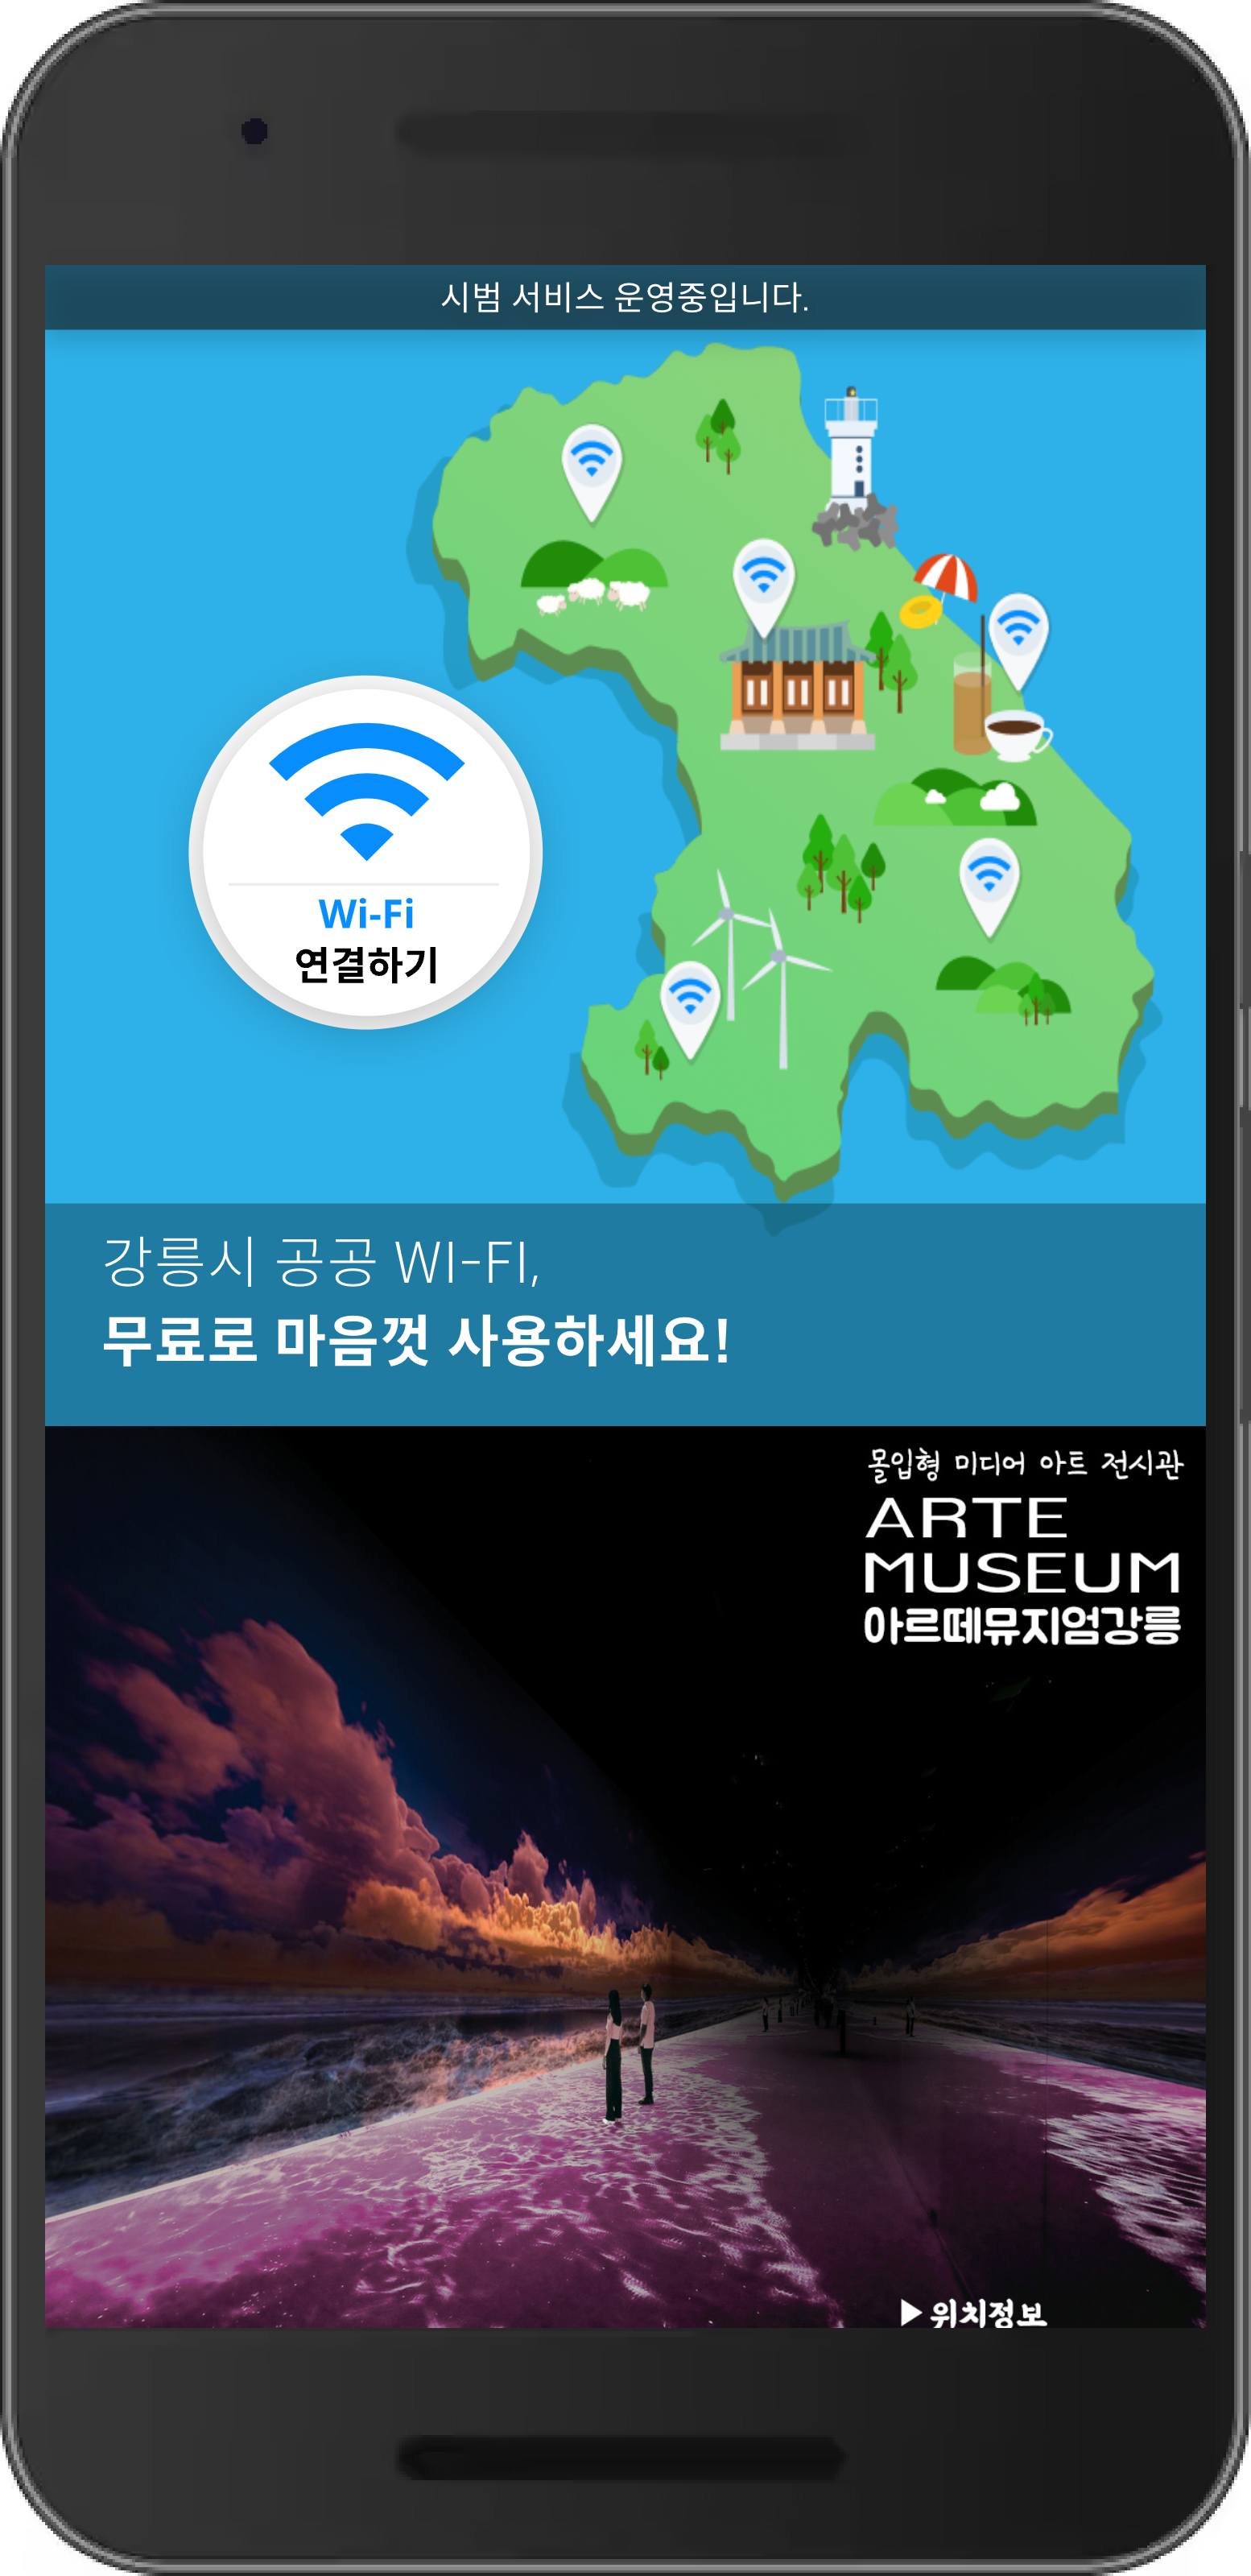
\includegraphics[width=0.3\textwidth]{images/public-ad-fi-gn-captiveportal.png}
					            \caption*{공공 WiFi Captive portal}
				            }
			            \end{fullwidth}
		            \end{figure}
	      \end{itemize}
	      \begin{figure}[!ht]
		      \begin{fullwidth}
			      \parbox{0.35\textwidth}{
				      \centering
				      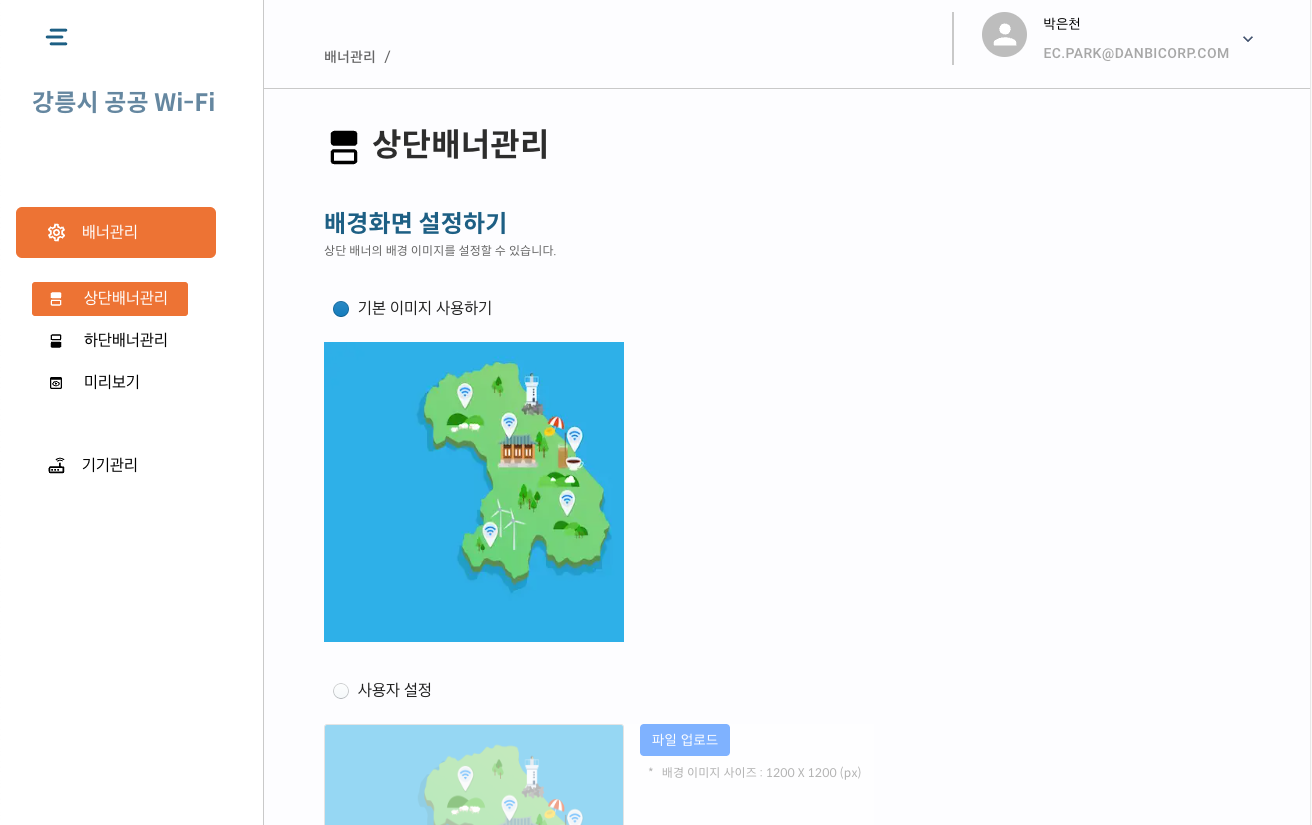
\includegraphics[width=0.35\textwidth]{images/public-ad-fi-upper-banner.png}
				      \caption*{상단배너 관리}
			      }\qquad
			      \parbox{0.35\textwidth}{
				      \centering
				      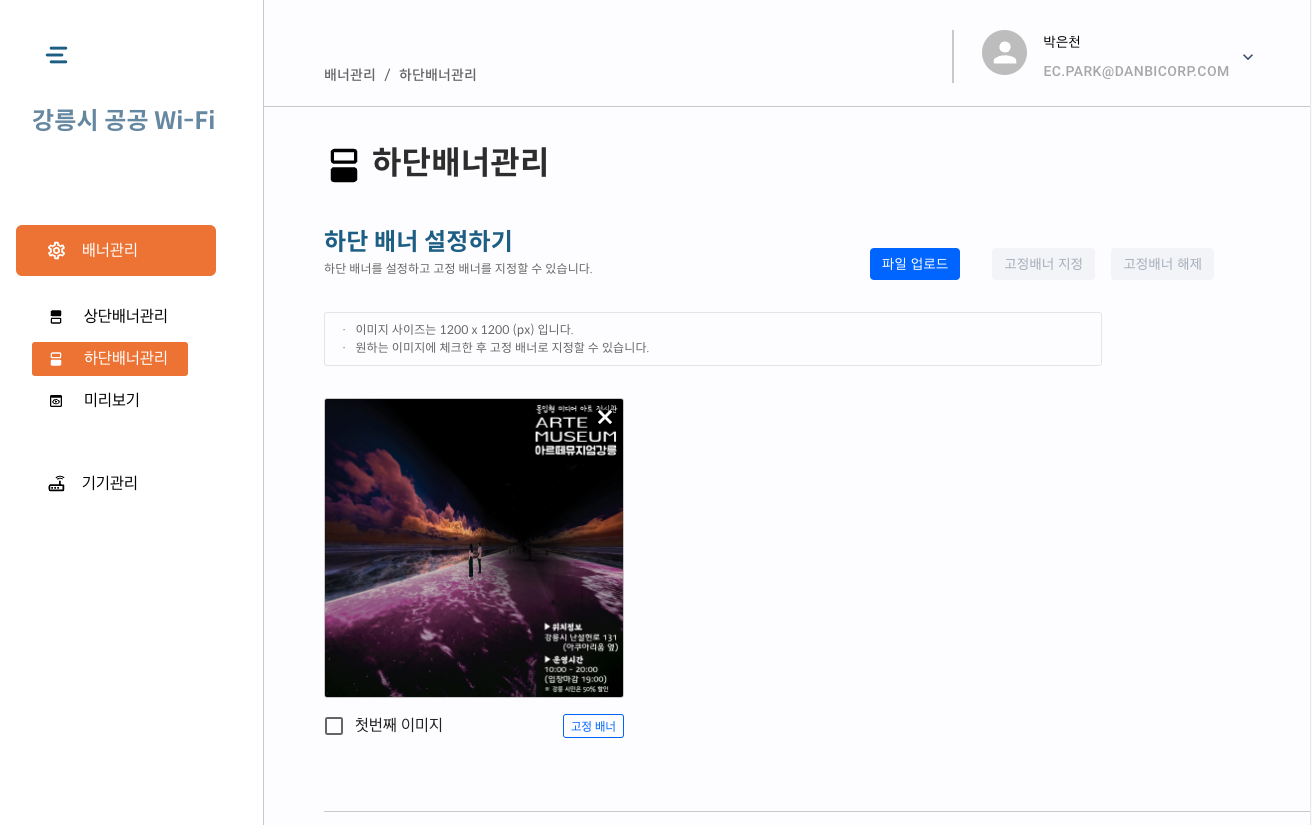
\includegraphics[width=0.35\textwidth]{images/public-ad-fi-lower-banner.png}
				      \caption*{하단배너 관리}
			      }\qquad
			      \parbox{0.35\textwidth}{
				      \centering
				      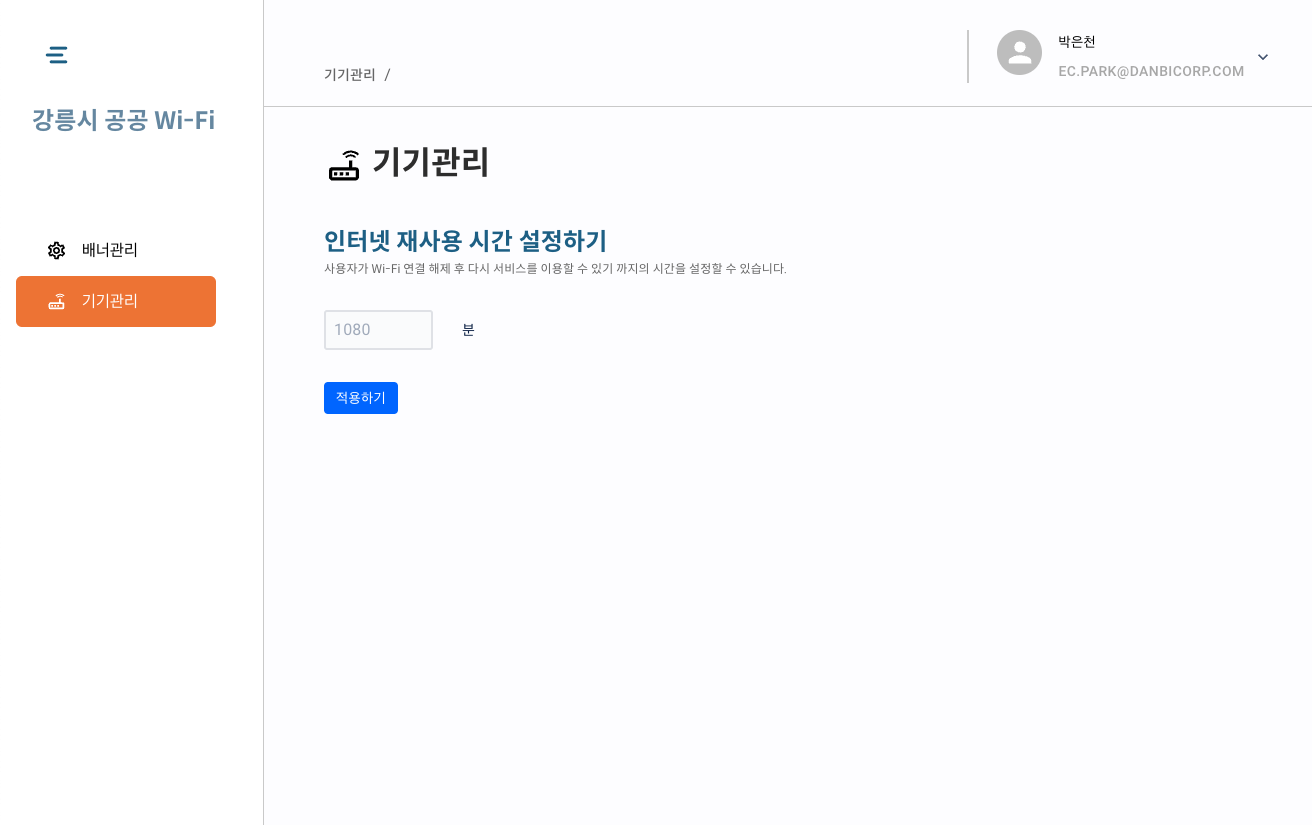
\includegraphics[width=0.35\textwidth]{images/public-ad-fi-device-manage.png}
				      \caption*{기기관리}
			      }\qquad
			      \parbox{0.35\textwidth}{
				      \centering
				      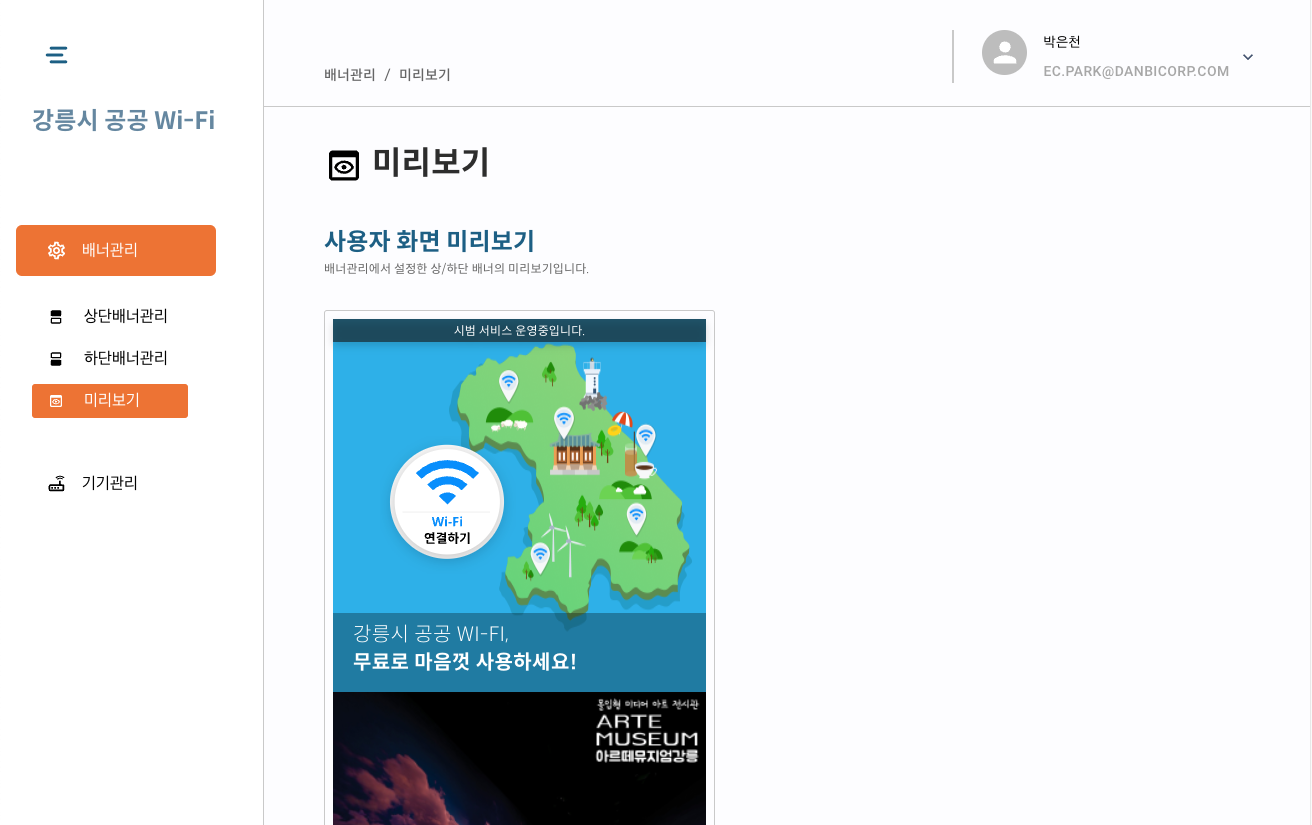
\includegraphics[width=0.35\textwidth]{images/public-ad-fi-preview.png}
				      \caption*{미리보기}
			      }
		      \end{fullwidth}
	      \end{figure}

\end{itemize}

\cvevent{\printinfo{\faPlusSquare}{Cash.Fi(매장 모객 서비스) 백엔드 개발}}{(주)단비코리아 개발리딩}{2021.06 -- 2021.06}{Seoul, Korea}

\label{cashfi}

\begin{figure}[!ht]
	\begin{fullwidth}
		\parbox{1.6\textwidth}{
			\centering
			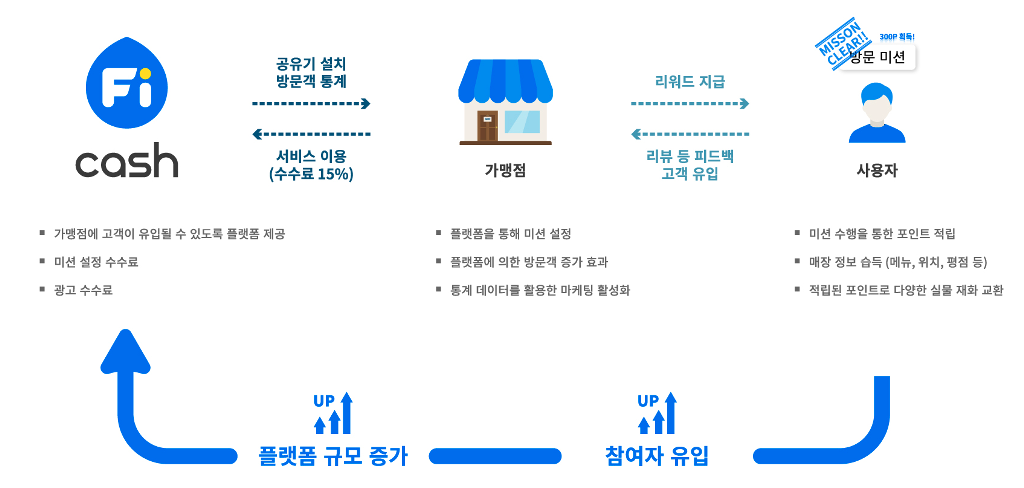
\includegraphics[width=0.5\textwidth]{images/cash-fi.png}
			\caption*{Cash Fi}
		}
	\end{fullwidth}
\end{figure}
\begin{itemize}[label=\emoji{satellite}]
	\item Cash.Fi(매장 모객 서비스) 백엔드 개발
	\item 총 개발 기간: 19개월 (외주 관리)
	\item 해당 개발 기간: 6주
	\item 개발 인력: 1인
	\item 개발한 서비스
	      \begin{itemize}[label=\emoji{pushpin}]
		      \item WiFi indoor position: WiFi 공유기와 Captive portal 연동, 매장 내부 위치 트래킹
		      \item WiFi 공유기 매장 fingerprint 수집: 공유기 AP를 이용 매장 특정 Fingerprint 개발(7종의 ML 알고리즘)
		      \item 외주 개발 백엔드 마이그레이션: DB 마이그레이션, AD-Fi 매장 연동
		      \item 인프라 구성: AWS EC2, RDS, S3, Lambda, CloudFront, Docker swarm stack: Traefik
		      \item 백엔드 스택: TypeScript, NodeJS, Express, Apollo Server, Prisma ORM
	      \end{itemize}

\end{itemize}